\documentclass[a4paper,8pt]{beamer} %{{{1
%\documentclass[a4paper,10pt]{thesis} 
%\documentclass[a4paper,9pt]{article} 
%\documentclass[a4paper,9pt]{article} 
\usepackage[utf8]{inputenc}

\usepackage{amsmath}
\usepackage{amsfonts}
\usepackage{amssymb}
%\usepackage{styfloats}
\usepackage{algorithmicx}
\usepackage{algorithm}  
\usepackage{algpseudocode}
\usepackage{subfigure}

\usepackage{listings}
\usepackage{cmap}
\lstset{breakatwhitespace,
language=C++,
columns=fullflexible,
keepspaces,
breaklines,
tabsize=3, 
showstringspaces=false,
extendedchars=true}

\usepackage{tikz}
\usetikzlibrary{shapes,arrows}

\usepackage{epsfig} %for å lime inn filer

%\usepackage{babel}  

\newcommand{\ts}[1]{\textbf{#1}}
\newcommand{\bra}[1]{\langle{#1}|}
\newcommand{\ket}[1]{|#1\rangle{}}
\newcommand{\abs}[1]{\left|{#1}\right|}
\newcommand{\sign}[1]{\text{sign}{#1}}
\newcommand{\diag}[1]{\text{diag}{#1}}
\newcommand{\ran}[1]{\text{ran}({#1})}
\newcommand{\norm}[1]{\lVert{#1}\rVert}

\newcommand{\smatrix}[1]{\left[\begin{matrix} #1 \end{matrix}\right]}

%\newtheorem{theorem}{Theorem}[subsection]
\newtheorem{algo}{Algorithm}%[section]
%\newtheorem{theorem}{Theorem}%[section]
%\newtheorem{lemma}[theorem]{Lemma}
%\newtheorem{proposition}[theorem]{Proposition}
%\newtheorem{corollary}[theorem]{Corollary}
%\newtheorem{assumption}[theorem]{Assumption}
%\newenvironment{proof}[1][Proof]{\begin{trivlist}
%\item[\hskip \labelsep {\bfseries #1}]}{\end{trivlist}}
%\newenvironment{definition}[1][Definition]{\begin{trivlist}
%\item[\hskip \labelsep {\bfseries #1}]}{\end{trivlist}}
%\newenvironment{example}[1][Example]{\begin{trivlist}
%\item[\hskip \labelsep {\bfseries #1}]}{\end{trivlist}}
%\newenvironment{remark}[1][Remark]{\begin{trivlist}
%\item[\hskip \labelsep {\bfseries #1}]}{\end{trivlist}}
%\newcommand{\qed}{\nobreak \ifvmode \relax \else
%      \ifdim\lastskip<1.5em \hskip-\lastskip
%      \hskip1.5em plus0em minus0.5em \fi \nobreak
%      \vrule height0.75em width0.5em depth0.25em\fi} 

% Define block styles
\tikzstyle{decision} = [diamond, draw, fill=blue!20, 
    text width=4.5em, text badly centered, node distance=1.8cm, inner sep=0pt]
\tikzstyle{block} = [rectangle, draw, fill=blue!20, 
    text width=12.5em, text centered, rounded corners, minimum height=4em]
\tikzstyle{line} = [draw, -latex']
%\tikzstyle{linebw} = [draw, latex-']
\tikzstyle{cloud} = [draw, ellipse,fill=red!20, node distance=3cm,
    minimum height=2em]

%\usepackagefig} %for å lime inn filer

%\usepackage{babel}  


%\usetheme[secheader]{Berlin}
%\usetheme[secheader]{umbc1}
%\usetheme[secheader]{Szeged}
%\usetheme[secheader]{Montpellier}
%\usetheme[secheader]{Berkeley}
\usecolortheme{rose}
%\usefonttheme{structuresmallcapsserif}
\usefonttheme{structurebold}
\begin{document}

%\title{Title}
%\author{Karl R. Leikanger}
%\affiliation{University of Oslo, Physics department}

%\maketitle
%\tableofcontents

%%%%%%%%%%%%%%%%%%%%%%%%%%%%%%%%%%%

\begin{frame}  %{{{1
\frametitle{INTRODUCTION:}
\begin{itemize}
\item The QR - algorithm for Hermitian matrices.
	\begin{enumerate}
		\item The QR - algorithm explained.
			\begin{enumerate}
				\item The Power Method.
				\item Orthogonal Subspace Iterations.
				\item The basic QR algorithm.
			\end{enumerate}
		\item Optimizations of the QR - algorithm.
			\begin{enumerate}
				\item Working with tridiagonal matrices.
				\item Explicit and implicit shifts
			\end{enumerate}
	\end{enumerate}
\item The SVD - algorithm. 
	\begin{enumerate}
		\item Basic idea.
		\item Optimizations: The Golub-Kahan algorithm
	\end{enumerate}
\end{itemize}
\end{frame} %}}}1 
\begin{frame}%{{{
	\frametitle{GENERAL QR - ALGORITHM}
	\begin{itemize}
		\item 
			The QR - algorithm is an iterative solver for eigen problems:
			\begin{align}
				Av=\lambda v.
			\end{align}
	\end{itemize}
\end{frame}%}}}
\begin{frame} %{{{1
\frametitle{THE GENERAL QR - ALGORITHM:}
%\begin{itemize}
%	\item 
The QR iteration algorithm $-$ same basic idea as the Power Method.
%\end{itemize}
%
%
\begin{columns}
%
%
\column{7cm}
\begin{itemize}
	\item<1-> Main idea: 
		\begin{enumerate}
			\item
				$A\in\mathbb C^n$: eigenvectors $\{v_i\}$, eigenvalues $\{\lambda_i\}$.
				\item 
					Set 
					\begin{align*}
						q^{(i+1)} = A q^{(i)} /  \norm{A q^{(i)}}_2
					\end{align*}
			\item 
				If $\max{}(\{|\lambda_i|\})=|\lambda_s|$ is non-degenerate then the sequence
				\begin{align*}
					\left\{ q^{(1)}, q^{(2)},\dots,q^{(N)} \right\},
				\end{align*}
				will converge to $v_s$
				given that $v_s^Tq\neq0$.
		\end{enumerate}
	\item<2-> What happens? Example: 
		\begin{enumerate}
			\item
				Assume that $A$ is normal. Then $A$ has the spectral decomposition
				\[ A = \sum_i\lambda_i v_iv_i^T \]
				and
				\[ q_N \propto A^Nq_0 = \sum_i \lambda_i^N (v_i^T q_0) v_i. \]
		\end{enumerate}
		%	\item Convergence proportional to (spesify) $\norm{\lambda_s}_2|/\norm{\lambda_t}_2$
		%		where $\lambda_t$ is the eigenvalue with the second largest magnitude.
\end{itemize}
%
%
\column{5cm}
\begin{algo}<3->
\begin{footnotesize}
{
%
	(The Power Method):
%
}\\
\textbf{Input: }
{
%
	\\$q^{(0)}\in\mathbb R^n$, $\norm{q}_2=1$.
	\\$A\in\mathbb R^{n\times n}$.
%
}\\
\textbf{Output: }
{
%
	\\One eigenvector $q^{(k)}$.
%
}\\
\line(1,0){120}
\begin{algorithmic}
%
\For{$k=1,2,3,\dots,k$}
	\State{$z\gets A q^{(k-1)}$}
	\State{$q^{(k)}\gets z/\norm{z}_2$}
	\State{$\lambda^{(k)} \gets [q^{(k)}]^T A q^{(k)}$}
\EndFor{}
%
\end{algorithmic}
\line(1,0){120}
\end{footnotesize}
\end{algo}
\end{columns}	
\end{frame} %}}}1
\begin{frame} %{THE GENERAL QR - ALGORITHM:} {{{1
\frametitle{THE GENERAL QR - ALGORITHM:}
%\begin{itemize}
%	\item 
The Power Method can be generalized to compute multiple eigenvectors.
%\end{itemize}
%
%
\begin{itemize}
	\item <1-> Main idea:
	\begin{enumerate}
		\item
		Power method with many vectors $q^{(k)}_1,q^{(k)}_2,\dots$ simultaneously. 
		\item	
		Orthonormalization each iteration s.t. 
		$q^{(k)}_1\gets q^{(k)}_1, q^{(k)}_2 \gets q^{(k)}_2 - q^{(k)}_1 {q^{(k)}_1}^Tq^{(k)}_2, \dots$
		\item Now, each $q_i^{(k)}$ will converge to an eigenvector.
		\item[-] 
		$q_1^{(k)}$: converges exactly in the same way as $q^{(k)}$ in the power method.
		\item[-]
		$q_2^{(k)}$ can be any vector $\in\ran{A}$ orthogonal to $q_1^{(k)}$
		$\Rightarrow$ it will converge to the eigenvector with the second largest eigenvalue. 
		\item[-]
		And so on....
	\end{enumerate}
	\item <2-> Orthonormalization is performed using the QR-factorization:
	\begin{footnotesize}
		\begin{align}
		& Q_{k} R_k \xleftarrow{\text{QR fact.}} A Q_{k-1} \quad\Rightarrow \notag \\
		& [q^{(k)}_1,q^{(k)}_2,\dots, q_n^{(k)}] 
		\smatrix{\times & \times & \times & \dots & \times \\ 
				0 		& \times & \times & \dots & \times \\
				0 		& 0 	& \times & \dots & \times \\
				\vdots  & 		& \vdots & 	& 	\vdots \\
				0 & 0 & \dots & 0 & \times }
		\xleftarrow{\text{QR fact.}} [ Aq^{(k-1)}_1, Aq^{(k-1)}_2,\dots, Aq_n^{(k-1)}] 
		\label{eq:qr}
		\end{align}
	\end{footnotesize}
\item <3-> As $Q_k$ converges s.t. $Q_k\approx Q_{k-1}$, $A = Q_kR_kQ_{k-1}^T \approx Q_k R_k Q_k^T$
will converge to Shur decomposition.
\end{itemize}
\end{frame} %}}}1
%\begin{frame} \frametitle{THE GENERAL QR - ALGORITHM:} %{{{1
%\begin{columns}
%%
%%
%\column{7cm}
%\begin{itemize}
%	\item 
%	If we assume that $\lambda_i>\lambda_{i+1}$ then 
%	the convergence of the $r$ first eigenvectors is proportional to $|\lambda_r/\lambda_{r+1}|$.
%	(Will be specified later).
%\end{itemize}
%%
%%
%\column{5cm}
%%%
%\begin{algo}
%{
%
%	(Orthogonal iteration):
%
%}\\
%\textbf{Input: }
%{
%%
%	\\$Q_0=I,\,Q_k\in\mathbb R^{n\times n}$.
%	\\$A\in\mathbb R^{n\times n}$.
%%
%}\\
%\textbf{Output: }
%{
%%
%	\\$\ran{Q_k(:,1:r)}=D_r(A)$ ($D=$ the dominant subspace of $A$ of dimension $r$).
%	\\The $r$ first diagonal elements of $T$ will converge to $(\lambda_1, \dots, \lambda_r)$.
%%
%}\\
%\line(1,0){120}
%\begin{algorithmic}
%%
%\For{$k=1,2,3,\dots,k$}
%	\State{$Z_k\gets A Q_{k-1}$}
%	\State{$Q_kR_k\gets Z_k$ (QR factorization)}
%\EndFor{}
%	\State{$T_k\gets Q^T_k A Q_k$ }
%%
%\end{algorithmic}
%\line(1,0){120}
%\label{algOrthoIi}
%\end{algo}
%%
%%
%%
%\end{columns}	
%\end{frame} %}}}1
\begin{frame}% {THE GENERAL QR - ALGORITHM:} {{{1
\frametitle{THE GENERAL QR - ALGORITHM:}
\begin{columns}
%
%
\column{7cm}
\begin{itemize}
%	\item (Nothing but an extension of orthogonal subspace iterations with $r=n$).
\item <1->
	In the QR-algorithm, $T_k=Q_k^TAQ_k$ is calculated directly, without explicitly multiplying with $A$.
	\begin{enumerate}
		\item[]
			We use Eq. \eqref{eq:qr} from the last slide.
			\begin{equation}
				Q_kR_k = AQ_{k-1} \Leftrightarrow R_kQ^T_{k-1} = Q_k^TA_k \notag\label{eq824_1} 
			\end{equation}
			Then
			\begin{align}
				&T_{k-1} = Q_{k-1}^T A Q_{k-1}  = Q_{k-1}^T Q_{k} R_{k} = \tilde Q_k R_k\label{eq824_2} \\
				&T_k = Q_k^T A Q_{k}  = R_k Q_{k-1}^T Q_{k} = R_k \tilde Q_k 	\notag\label{eq824_3} 
			\end{align}
	\end{enumerate}
\item <2-> If $A$ is normal, $T_k$ will converge to $\diag(\lambda_1,\lambda_2,\dots,\lambda_n)$.
\end{itemize}	

\column{5cm}
%
%
\begin{algo} <3->
\begin{footnotesize}
{
%
	(QR iteration):
%
}\\
\textbf{Input: }
{
%
	\\$Q_0=I,\,Q_0\in\mathbb R^{n\times n}$.
	\\$A\in\mathbb R^{n\times n}$.
%
}\\
\textbf{Output: }
{
%
	\\$T_k$ contains the eigenvalues of $A$ (Highest magnitude first). 
	\\$Q_ke_i$ is the $i$'th eigenvector of $A$.
%
}\\
\line(1,0){120}
\begin{algorithmic}
%
\State{$T_0\gets \tilde Q_0^T A \tilde Q_{0}$}
\For{$k=1,2,3,\dots,k$}
	\State{$\tilde Q_kR_k\gets T_{k-1}$ (QR factorization)}
	\State{$T_k\gets R_{k}\tilde Q_{k-1}$}
\EndFor{}
%
\end{algorithmic}
\line(1,0){120}
\label{algQRIterSimple}
\end{footnotesize}
\end{algo}
%
%

\end{columns}
\end{frame} %}}}1
\begin{frame}[label=framelb1]  %{{{1
\frametitle{THE QR - ALGORITHM FOR HERMITIAN MATRICES }
\begin{itemize}
\item <1-> The performance of the above QR - Algorithm is poor:
	\begin{enumerate}
		\item Each iteration is $\mathcal O(n^3)$.
		\item The convergence can be very slow if the modulus of a pair of eigenvalues are close
		\[ \text{dist}(\text{span}(q_1^{(k)},q_2^{(k)},\dots,q_{n-1}^{(k)})
			,\text{span}(q_1,q_2,\dots,q_{n-1})) \propto \mathcal O(|\lambda_{n}/\lambda_{_n+1}|)^k \]
		(ref:G\&L p. 411)	
		\hyperlink{dist span}{\beamergotobutton{(*)}}
	\end{enumerate}
\item <2-> When $A$ is Hermitian, the convergence can be considerably improved by:
	\begin{enumerate}
		\item Reducing $A$ to a symmetric tridiagonal real matrix $T$.
		\item Introducing single shifts. 
	\end{enumerate}
\end{itemize}
\end{frame} %}}}1
\begin{frame}[label=tridiagonalizationofa]  %{{{1
\frametitle{TRIDIAGONALIZATION OF A}
Reduction to symmetric tridiagonal form:
\begin{itemize}
	\item <1-> Any Hermitian matrix $A^\dagger = A$ is unitarily similar to a real symmetric tridiagonal matrix:
\begin{equation}
H^\dagger AH = T,\, 
T=
	\smatrix{
		a_1 & b_1 & & & 0\\
		b_1 & a_2 & b_2 & & \\
		& b_2 & a_3 & \ddots & \\
		& & \ddots	& \ddots & b_{n-1} \\
		0& & & b_{n-1}& a_n 
	}
	\, a_i, b_i \in \mathbb R.
\end{equation}
	\item <2->
		The Householder reduction to tridiagonal form reqiures $ 4/3 n^3$ flops, and reduces the cost of the 
		QR - iterations from an $\mathcal O(n^3)$ operation to an $\mathcal O(n)$ operation. 
		($\mathcal O(n^2)$ if the rotations are accumulated).
	\item  <3->
		$T$ and $A$ has the same eigenvalues, while the eigenvectors 
		is different. In general, if $Tv_i = \lambda_iv_i$, then $A H^T v_i = \lambda_i H^Tv_i$.
\end{itemize}	
\begin{footnotesize}
	[Householders transformations:] %(Show stepwise with illustrations). 
	\hyperlink{householders explained}{\beamergotobutton{(*)}} 
\end{footnotesize}
	%\[ HAH^T = T ,\, T\in\mathbb R^n\]
\end{frame} %}}}1
\begin{frame}  %{{{1
\frametitle{INTRODUCING SHIFTS}
\begin{columns}

\column{7cm}
\begin{itemize}
	%\item Assume that $\lambda(T) = \{\lambda_1,\lambda_2,\dots,\lambda_n \}$.
	%and that $\lambda_i\ge\lambda_{i+1}$. 
	\item <1-> We can shift all the eigenvalues $\lambda_i\gets\lambda_{i}-s$ 
	by setting $T\gets T-sI$.
	\item <2->
	If $s$ is close to an eigenvalue then 
	$T_{n-1,n}$ will be small after a $QR$ step with shift $s$. 
	\begin{enumerate}
	%This can be made very intuitive if we remember from the QR algorithm 
	%that the 
	\item[]<3->
	Convergence %towards the eigenvectors 
%	\begin{equation}
%		\text{span} \dots \dots
%		v_1,\dots,v_{n-1} \gets
%		q^{(k)}_1,\dots,q^{(k)}_{n-1}
%	\end{equation}
	proportional to $|\lambda_{n}/\lambda_{n-1}|$.
	If $s\approx\lambda_{n}$, we increase the ratio
	between the eigenvalues and thereby accelerate the convergence. 
	\end{enumerate}
	\item <4-> Wilkinson Shifts: The eigenvalue of the $2\times2$ block $T(n:n+1, n:n+1)$, which
	is closest to $T{n+1,n+1}$. %because of the tridiagonal form of T.
\end{itemize}

\column{5cm}
%
%
\begin{algo} <4->
\begin{footnotesize}
{
%
	(Explicit Single Shift QR):
%
}\\
\textbf{Input: }
{
%
	\\The symmetric and tridiagonal matrix $T\in\mathbb R^{n\times n}$.
%
}\\
\textbf{Output: }
{
%
	\\$T$ as the Shur decomposition.
	\\$Q$ where $Qe_i$ is the $i$'th eigenvector.
%
}\\
\line(1,0){120}
\begin{algorithmic}
%
\State{$T=U_0^TAU_0$}
\For{k=1,2,\dots}
	\State{Determine the shift $s\in\mathbb R$}
	\State{$UR\gets T-sI$ (QR-factorization)}
	\State{$T\gets RU+sI$}
\EndFor{}
%
\end{algorithmic}
\label{algQRSingleShiflExplicit}
\line(1,0){120}
\end{footnotesize}
\end{algo}
%\end{algorithm} 
%
\end{columns}
\end{frame} %}}}1
\begin{frame}  %{{{1
\frametitle{THE QR ALGORITHM WITH EXPLICIT SHIFTS}
\begin{itemize}
\item <1-> Example: The Wilkinson shift of the last block is used.
\begin{tiny}
\begin{align}
&A = \smatrix{
   4.0000  & 1.0000 &       0  &      0 \\
   1.0000  & 3.0000 &  2.0000  &      0 \\
        0  & 2.0000 &  2.0000  & \ts{3.0000} \\
        0  &      0 &  \ts{3.0000}  & 1.0000 }
,\,\notag\\
&T_1 = \smatrix{
   4.3180 & 0.8409 &      0 &      0\\
   0.8409 & 4.0675 &-1.6172 &      0\\
        0 &-1.6172 & 3.4988 &\ts{-0.4325}\\
        0 &      0 &\ts{-0.4325} &-1.8842}
,\,\notag\\
&T_2 = \smatrix{
   4.5362  & 0.8071  &      0 &       0\\
   0.8071  & 4.6509  &-1.2878 &       0\\
        0  &-1.2878  & 2.7347 &  \ts{0.0003}\\
        0  &      0  & \ts{0.0003} & -1.9218}
,\,\notag\\
&T_3 = \smatrix{
   4.7366 &  0.81226e  &      0  &      0\\
   0.81226 &  4.8769  &-0.84826  &      0\\
        0 & -0.84826  & 2.3083  &\ts{-6.1489e-14}\\
        0 &       0  &\ts{-6.1489e-14}  &-1.9218}
\end{align}
Eigenvalues: $\{5.7424, 4.1477, 2.0317, \ts {-1.9218} \}$
\end{tiny}
\item <2-> The Wilkinson shift is a better approximation to $\lambda_{n}$ the smaller
	the off diagonal elements gets $\Rightarrow$ The convergence bets better for each iteration.
\end{itemize}
\end{frame} %}}}1
\begin{frame}  %{{{1
\frametitle{THE QR ALGORITHM WITH EXPLICIT SHIFTS}
\begin{itemize}
	\item <1-> Error analysis:
		\begin{enumerate}
	%		\item Error of a single QR - transformation
	%			(G\&L p.225):\\
	%			\begin{quote}
	%				The computed upper triangular matrix $\tilde R$ is the exact $R$ for a nearby $A$
	%				in the sense that $Z^T(A+E)=\tilde R$ where $Z$ is some exact orthonormal matrix
	%				and $\norm{E}_2\approx\ts u\norm{A}_2$.
	%			\end{quote}
			\item From Corollary 8.1.6 in G\&L: %The error $\lambda_k(A+E)-\lambda_k(A)$ is
				\begin{equation}
					%|\lambda_k(A+E)-\lambda_k(A)| \le \ts u\norm{A}_2 
					|\tilde \lambda_k(A)-\lambda_k(A)| \le \ts u\norm{A}_2 
				\end{equation}
		\end{enumerate}
	\item <2-> The eigenvalues are calculated with the same absolute error, meaning that the 
			smaller eigenvalues will have a larger relative error.
\end{itemize}
\end{frame} %}}}1
\begin{frame}%{{{
	\frametitle{THE EXPLICIT QR ALGORITHM}
\begin{itemize}
	\item <1-> Problem: If the shifts are large compared to some of the diagonal elements, 
				a QR-step with a large shift might degrade some of the smaller eigenvalues (ref art).
	\item <2-> Example:
		\begin{enumerate}
			\item <2->
				Consider for example a matrix A with elements of the orders of
				magnitude given by
				\begin{align}
					A= \smatrix{
						1&1&0&0\\
						1&10^{2}&10^{1}&0\\
						0&10^{1}&10^{4}&10^{2}\\
						0&0&10^{2}&10^{7}\\
					}
				\end{align}
				which has eigenvalues of orders $\{1,10^2,10^4,10^{7}\}$. 
			\item <3-> In float arithmethics: After the first QR - step, 
				the first diagonal element is 0 for $A_{11}\in(-5,5)$.
			\item <4-> A lot of round off error!
				%The first shift determined from the last $2\times 2$ matrix is then obviously of 
				%order $10^{12}$. Suppose we are
				%using a $10$ digit decimal computer. When the shift is subtracted from $A_{11}$,
				%small eigenvalue, which is well determined by the data, is inevitably lost. In this example the
				%difficulty could be avoided by reflecting the matrix in the secondary diagonal.
		\end{enumerate}
	\item <5-> Solution: Implicit shifts.
\end{itemize}
\end{frame}%}}}
\begin{frame} % {{{1
	\frametitle{THE QR ALGORITHM WITH IMPLICIT SHIFTS}
		\begin{itemize}
				\item <1->
		Note that the shifted QR-step is an unitary operation:
		\begin{equation}
			\left.
			\begin{matrix}
				Q_kR\gets T_{k}-sI\\
				T_{k+1}\gets RQ_k + sI
			\end{matrix}
			\right\} \text{ equivalent to }  T_{k+1} \gets Q_k^T (T_k - s I ) Q_k + sI =  Q_k^T T_k Q_k 
		\end{equation}
	\item <2-> The implicit Q-theorem:  
		\begin
		{theorem}[The Implicit Q-Theorem]
			\begin{tiny}
				Suppose $Q=(q_1,q_2,\dots,q_n)$ and $V=(v_1,v_2,\dots,v_n)$ are orthogonal matrices with the property
				that both $Q^TAQ=T$ and $V^TAV=S$ are tridiagonal where $A\in\mathbb R^{n\times n}$ is symmetric.
				Let $k$ denote the smallest index where $T_{k+1,k}=0$, with the convention that $k=n$ is $T$ is 
				unreduced. If $v_1=q_1$ than $v_i=\pm q_i$ and $T_{i,i-1} = S_{i,i-1}$ for $i=2:k$. Moreover, if
				$k<n$, then $S_{k+1,k}=0$.
			\end{tiny}
		\end{theorem}
	\item <3-> Meaning that:
		\begin{enumerate}
			\item <3-> If we can find an $U$ s.t. $U^TTU$ is on tridiagonal form and $Ue_1=Q_ke_1$, then
				$Q_k^TT_kQ_k = DU^TT_kUD$ where $U=\diag(\pm1,\pm1,\dots,\pm1)$.
			\item <4-> The small offdiagonal elements in $Q_k^{T}TQ_k$ will be small in $U^{T}T_kU$ as well!
		\end{enumerate}
		\end{itemize}
\end{frame} %}}}1
\begin{frame} %{{{
\frametitle{THE QR ALGORITHM WITH IMPLICIT SHIFTS:} 
	\begin{itemize}
		\item
		We want to form a matrix $U$ which is a product of Givens transformations
		\begin{align}
			&U = U_{1}U_{2}\dots U_{n-1}, \notag\\ 
			&U_i = 
			\smatrix{ 
				I^{i-1\times i-1} 	& 0 	& 0 \\ 
				0 					& G_i 	& 0 \\ 
				0 					& 0 	& I^{n-i-2\times n-i-2}}, \notag\\
				&G_i = \smatrix{cos(\theta_i) & \sin(\theta_i) \\ -\sin(\theta_i) & \cos(\theta_i)}
		\end{align}
		where the first column of $U$ is equal to the first column of $Q_k$.
		\item
		note that $Ue_1 = U_1e_1 = \smatrix{cos(\theta_1)\\ -\sin(\theta_1) \\ 0 \\ 0 \\ \vdots}$
	\end{itemize}
\end{frame}%}}}1
\begin{frame}  %{{{1
\frametitle{THE QR ALGORITHM WITH IMPLICIT SHIFTS:}
	\begin{itemize}
		\item
			To find a $U$ s.t. $Q_ke_1=Ue_1$ we must find a $\theta_1$ such that
			\begin{equation}
				G_1 
				\smatrix{ T_{11}-s \\ T_{21} } \propto \smatrix{ 1 \\ 0} = 
	%\smatrix{ \cos(\theta_1) & \sin(\theta_1) \\ -\sin(\theta_1) & \cos(\theta_1) } 
	%\smatrix{ T_{11}-s \\ T_{21} } \propto \smatrix{ 1 \\ 0} \label{eq835}. 
				\Rightarrow
				G_1 \propto  \smatrix{T_{11}-s & -T_{21} \\ T_{21} & T_{11}-s}
				\Rightarrow
				Ue_1 \propto \smatrix{T_{11}-s\\T_{21} \\0\\0\\ \vdots}
			\end{equation}
		\item
			Correct since
			\begin{equation}
				Q_kRe_1 = \smatrix{T_{11}-s\\T_{21}\\0\\0\\ \vdots} 
				\Rightarrow Q_ke_1 \propto  \smatrix{T_{11}-s\\T_{21} \\0\\0\\ \vdots}
			\end{equation}
			because $R$ is upper triangular. Then
		\item
			Since both $Q_k$ and $U$ is orthogonal, the proportionalities implies that 
			the first column of $Q_k$ and $U$ is equal.
	\end{itemize}
\end{frame}%}}}1
\begin{frame}  %{{{1
\frametitle{THE QR ALGORITHM WITH IMPLICIT SHIFTS:}
\begin{itemize}
	\item
	The next step is to show how $G_i,\,i>1$ can be constructed such that $U^TTU$ is tridiagonal.
	First, look at this example where $T$ is an $5\times 5$ matrix.
	\begin{equation}
		\begin{footnotesize}
		T'=U_1 ^T T U_1= 
		\smatrix
		{
			\times 	& \times & + & 0 & 0   \\
			\times 	& \times & \times & 0 & 0   \\
			+   	& \times & \times & \times & 0   \\
			0 & 0 & \times & \times & \times     \\
			0 & 0 & 0 & \times & \times    \\
		}
		,\,
		T''=U_2^T T' U_2 = 
		\smatrix
		{
			\times 	& \times & 0 & 0 & 0   \\
			\times 	& \times & \times & + & 0   \\
			0 	& \times & \times & \times & 0    \\
			0 & + & \times & \times & \times   \\
			0 & 0 & 0 & \times & \times  \\
		}
		\end{footnotesize}
	\end{equation}
		%,\notag\\
	\begin{equation}
		\begin{footnotesize}
		U'''=U_3^T T'' U_3 = 
		\smatrix
		{
			\times 	& \times & 0 & 0 & 0   \\
			\times 	& \times & \times & 0 & 0   \\
			0 	& \times & \times & \times & +\\
			0 & 0 & \times & \times & \times   \\
			0 & 0 & + & \times & \times  \\
		}
		,\,
		T''''=U_4^{T}T'''U_4= 
		\smatrix
		{
			\times 	& \times & 0 & 0 & 0   \\
			\times 	& \times & \times & 0 & 0   \\
			0 	& \times & \times & \times & 0    \\
			0 & 0 & \times & \times & \times   \\
			0 & 0 & 0 & \times & \times  \\
		}
		.
		\end{footnotesize}
	\end{equation}
\item $\Rightarrow U = U_{4}U_{3}U_{2}U_{1}$ will bring $T$ on tridiagonal form.
\end{itemize}
\end{frame}%}}}1
\begin{frame} \frametitle{THE QR ALGORITHM WITH IMPLICIT SHIFTS:} %{{{1
		The $G_i$'s can be found by solving the following equation
		\begin{align}
			\smatrix{
				1 & 0 & 0 & 0 \\
				0 & c & -s & 0 \\
				0 & s & c & 0 \\
				0 & 0 & 0 & 1 
			}
			\smatrix{
				a_i& b_i & z_i & 0 \\
				b_i & a_p & b_p & 0 \\
				z_i & b_p & a_q & b_p \\
				0 & 0 & b_q & a_r 
			}
			\smatrix{
				1 & 0 & 0 & 0 \\
				0 & c & s & 0 \\
				0 & -s & c & 0 \\
				0 & 0 & 0 & 1 
			}
			=
			\smatrix{
				\tilde a_i& \tilde b_i & 0 & 0 \\
				\tilde b_i &\tilde a_p &\tilde b_p &\tilde z_p \\
				0 &\tilde b_p &\tilde a_q &\tilde b_p \\
				0 &\tilde z_p &\tilde b_q &\tilde a_r 
			}
		\end{align}
		where $(p,q,r)=(i+1, i+2, i+3)$. We simply need to find a $b_is+z_ic = 0$
		and then to explicitly do the transform. 
		%$G_i$ can be written 
%\begin{align}
%	G_i = \frac1{N}\smatrix{ 1 & \frac{z_i}{b_i} \\ -\frac{z_i}{b_i} & 1 }
%	\text{ where } N = \left[\frac{z_i}{b_i}\right]^2+1.
%\end{align}
	\end{frame}%}}}1
\begin{frame} %{{{
\frametitle{THE QR ALGORITHM WITH IMPLICIT SHIFTS:} 
\begin{itemize}
	\item deflation = speedup. Ex: 3 givens rotations $+$ formation of $G_1$.
		\begin{align}
			T_k = \smatrix{
				\times & \times & 		0 	& 0 & 0 & 0 \\
				\times & \times & \times 	& 0 & 0 & 0 \\
				0 & \times & \times	& \times 	& 0 & 0 \\
				0 &  0 & \times	& \times 		& 0 & 0 \\
				0 &  0 & 0	& 0 	& \times & 0 \\
				0 &  0 & 0	& 0 	& 0 & \times \\
			}
		\end{align}
	\item $D_k$ on reduced tridiagonal form = speedup. 2 givens rotations $+$ formation of $G_1$.
		\begin{align}
			T_k = \smatrix{
				\times & 0 & 		0 	& 0 & 0 & 0 \\
				0 & \times & \times 	& 0 & 0 & 0 \\
				0 & \times & \times	& \times 	& 0 & 0 \\
				0 &  0 & \times	& \times 		& 0 & 0 \\
				0 &  0 & 0	& 0 	& \times & 0 \\
				0 &  0 & 0	& 0 	& 0 & \times \\
			}
		\end{align}
\end{itemize}
\end{frame}%}}}1
\begin{frame} %{{{
\frametitle{THE QR ALGORITHM WITH IMPLICIT SHIFTS:}
\begin{algo}[Symmetric QR Algorithm]
\begin{footnotesize}
\textbf{Input: }
{
%
The hermitian matrix $A\in\mathbb R^{n\times n}$, 
%
}
\textbf{Output: }
{
%
$T$ as the Shur decomposition.
%
}\\
\line(1,0){120}
\begin{algorithmic}
%
\State{Compute the tridiagonalization $T\gets A$:}
	\State{\hspace{4mm} $T=(P_1\dots P_n-2)^TA(P_1\dots P_n-2)$}
	\State{\hspace{4mm} Set $D=T$ and form $Q=P_1\dots P_n$ if $Q$ is desired.}
\While{$q<n$}
	\For{$i=1:n-1$}
		\If{$|d_{i+1,i}|$ and $|d_{i,i+1}|$ $\le\text{tol}(|d_{ii}|+|d_{i+1,i+1}|)$}
			\State{$d_{i,i+1}\gets0$}
			\State{$d_{i+1,i}\gets0$}
		\EndIf{}
	\EndFor{}
	\State{Find the largest $q$ and the smallest $p$ such that if
		\begin{equation}
		D = 
		\begin{matrix}
			\\
			\smatrix{D_{11} & 0 & 0 \\ 0 & D_{22} & 0 \\ 0 & 0 & D_{33}} 
			& 
			\begin{matrix}
				p \\ n-p-q \\ q
			\end{matrix}
			\\
			\begin{matrix}
				p & n-p-q & q
			\end{matrix}
		\end{matrix},
		\end{equation}
		}
		\State{then $D_{33}$ is diagonal and $D_{22}$ is unreduced.}
	\If{$q<n$}
		\State{Apply a single implicitly shifted QR-Step to $D_{22}:$}
		\State{\hspace{4mm}$D=\text{diag}(I_p,\overline Z, I_q)^T D\text{diag}(I_p,\overline Z, I_q) $}
		\State{If $Q$ is desired, then let $Q=Q\text{diag}(I_p,\overline Z, I_q)  $}
	\EndIf{}
\EndWhile{}
%
\end{algorithmic}
\label{algQRAlgorithm}
\line(1,0){120}
\end{footnotesize}
\end{algo}
\end{frame}%}}}1
\defverbatim[colored]\lst{%%{{{
	\begin{TINY}
		\begin{lstlisting}[tabsize=8,basicstyle=\ttfamily]
		void implicitQRstep(colvec &c_a, colvec &c_b, const int in, const int ir)
		{
			.....
			//find the Wilkinson shift (the eigenvalue of the last block)
			.....	
			//do the first givens rotation
			.....	
			if (in-ir>2) //if !(ir-in>2) the above rotation yields the exact answer
			{
				c_b[ir+1]   = d_bkp1*dc;
				d_z         = - d_bkp1*ds;

				//do the rest of the givens rotations except the last
				for (k=ir+1; k<in-2; k++)
				{
					d_ak    = c_a(k);
					d_akp1  = c_a(k+1);
					d_bkm1  = c_b(k-1);
					d_bk    = c_b(k);
					d_bkp1  = c_b(k+1);

					givens(dc, ds, d_bkm1, d_z);

					c_b(k-1)    = d_bkm1*dc - d_z*ds;
					c_a(k)      = dc*dc*d_ak - 2.0*ds*dc*d_bk + ds*ds*d_akp1;
					c_a(k+1)    = ds*ds*d_ak + 2.0*ds*dc*d_bk + dc*dc*d_akp1;
					c_b(k)      = ds*dc*(d_ak - d_akp1) + d_bk*(dc*dc - ds*ds);
					c_b(k+1)    = dc*d_bkp1;
					d_z         = - d_bkp1*ds;
				}
				//do the last givens rotation
				.....	
			}
		}
		\end{lstlisting}
	\end{TINY}
}

\begin{frame}
	\frametitle{THE QR ALGORITHM WITH IMPLICIT SHIFTS}
	\begin{itemize}
		\item The single implicit QR-step:
			\begin{enumerate}
				\item Only 2 vectors of length $n$ in memory.
				\item Approx $n\times 50$ flops.
			\end{enumerate}
		\lst
	\end{itemize}
\end{frame}%}}}
\begin{frame} %{{{1
\frametitle{CONVERGENCE AND ERROR}
\begin{columns}%
\column{6cm}
\begin{figure}%{{{3
\begin{center}
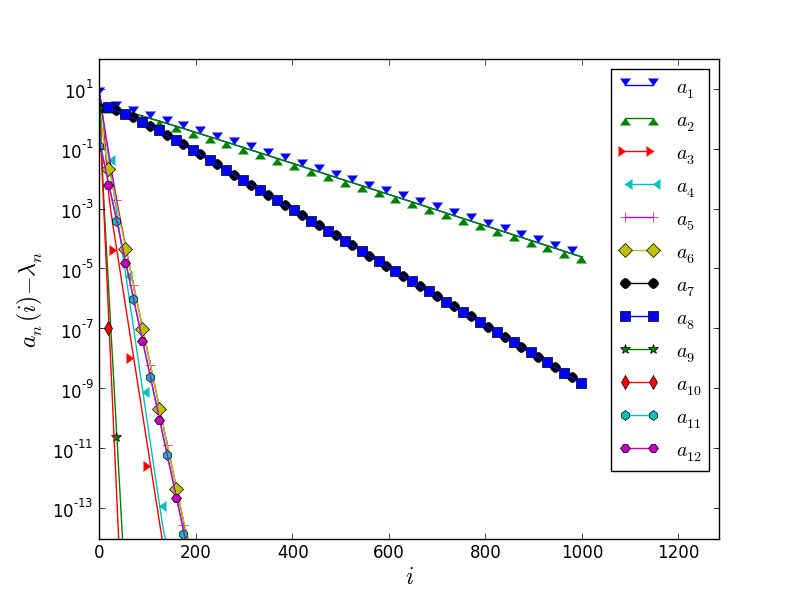
\includegraphics[height=3.8cm]{12x12randn_eigv_conv_QRstandard.png}
	\begin{scriptsize}
	\begin{tabular}{ll}
		\hline
		\hline
		\\
		$\lambda_1=
		-6.544395991691173
		$ & $\lambda_2=
		6.583845448270952
		$ \\ $\lambda_3=
		-4.759692498020273
		$ & $\lambda_4=
		4.227228411195598
		$ \\ $\lambda_5=
		-3.718806489258647
		$ & $\lambda_6=
		3.406092305333206
		$ \\ $\lambda_7=
		-2.508608861858869
		$ & $\lambda_8=
		2.480820818364306
		$ \\ $\lambda_9=
		-1.768319271480477
		$ & $\lambda_{10}=
		0.731101702075869
		$ \\ $\lambda_{11}=
		-0.4860591502185416
		$ & $\lambda_{12}=
		0.4459711429826421
		$ \\
		\\
		\hline
		\hline
	\end{tabular}
	\end{scriptsize}
\caption{
	The basic QR- algorithm without shifts. The convergence of the leading principal submatrix
	of dimension $k$ is $\propto |(\lambda_k/\lambda_{k+1})|^i$
}
\end{center}
\end{figure}
%
%
%
\column{6cm}
%
\begin{figure}
\begin{center}
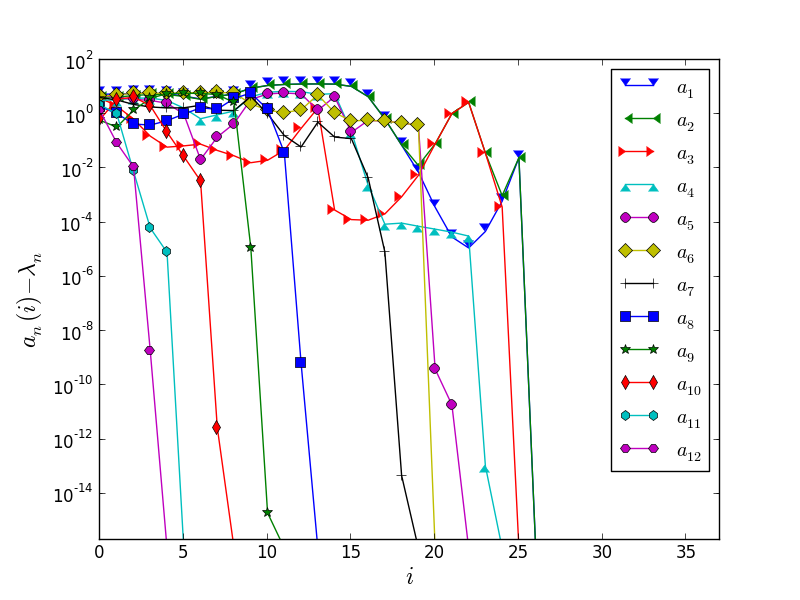
\includegraphics[height=3.8cm]{12x12randn_eigv_conv_QRfull.png}
	\begin{scriptsize}
	\begin{tabular}{ll}
		\hline
		\hline
		\\
		$\lambda_1=
		-6.544395991691173
		$ & $\lambda_2=
		6.583845448270952
		$ \\ $\lambda_3=
		-4.759692498020273
		$ & $\lambda_4=
		-3.718806489258647
		$ \\ $\lambda_5=
		2.480820818364306
		$ & $\lambda_6=
		4.227228411195598
		$ \\ $\lambda_7=
		3.406092305333206
		$ & $\lambda_8=
		-2.508608861858869
		$ \\ $\lambda_9=
		-1.768319271480477
		$ & $\lambda_{10}=
		-0.4860591502185416
		$ \\ $\lambda_{11}=
		0.731101702075869
		$ & $\lambda_{12}=
		0.4459711429826421
		$ \\
		\\
		\hline
		\hline
	\end{tabular}
	\end{scriptsize}
\caption{
	The full implicit QR- algorithm with Wilkinson shifts and deflation. Quadratic convergence
	of the shifted eigenvalue. 
}
\end{center}
\end{figure}
%
%
%
\end{columns}
\end{frame}%}}}1
\begin{frame} %{{{
\frametitle{OVERVIEW:}
		\begin{itemize}
			\item Tridiagonalization algorithms:
				\begin{table}
					\begin{Tiny}
						\centering
						\begin{tabular}{lll}
							\hline
							\hline
							\\
							Method & Cost (With unitary mat.) & Convergence (Without Unitary mat.) \\
							\\
							\hline
							\\
							Householders tridiagonalization (dense matrices) 	& $4n^3/3 $ & $ 8n^3/3 $ \\
							Givens tridiagonalization (dense matrices)			& %$4n^3/3$ 
							 &  \\
							Lanczos tridiagonalization (sparse matrices)		& & \\
							\\
							\hline
							\hline
						\end{tabular}
					\end{Tiny}
				\end{table}
			\item Eigen solvers for real symmetric tridiagonal matrices:
				\begin{table}
					\begin{Tiny}
						\centering
						\begin{tabular}{llll}
							\hline
							\hline
							\\
							Method & Output & Cost/Iteration & Convergence \\
							\\
							\hline
							\\
							Inverse iteration 			& $v_i$ (with imput $\lambda_{i})$ & $\mathcal O(n)$ (for tridiag. mat.) & Linear\\ 
							Rayleigh quotient iteration & $v_i$, $\lambda_{i}$ & $\mathcal O(n)$ &	Cubic \\
							Bisection (Sturm Sequence) method 	& The required $\lambda_i$ 	& $\mathcal O(n^2)$ & Linear \\
							Bisection method 		& a $\lambda_i$ in a given interval.	& $\mathcal O(n)$ & Linear \\
							QR algorithm 				& $\{\lambda_i\}$ and $\{v_i\}$ or only $\{\lambda_i\}$ & $\mathcal O(n^2)$ or $\mathcal O(n)$ & Cubic\\
							Divide-and-conquer 			& $\{\lambda_i\}$ 	&  & \\
							\\
							\hline
							\hline
						\end{tabular}
					\end{Tiny}
				\end{table}
			\item Eigen solvers for symmetric matrices:
				\begin{table}
					\begin{Tiny}
						\centering
						\begin{tabular}{llll}
							\hline
							\hline
							\\
							Method & Output & Cost/Iteration & Convergence \\
							\\
							\hline
							\\
							Power iteration 			& $v_i, \lambda_{i}=\max{(\{\lambda_i\})}$ & $\mathcal O(n^{2})$& Linear\\ 
							Inverse iteration 			& $v_i$ (with imput $\lambda_{i})$ & $\mathcal O(n^2)$ & Linear\\ 
							Rayleigh quotient iteration & $v_i$, $\lambda_{i}$ & $\mathcal O(n^2)$ &	Cubic \\
							Bisection method 		& a $\lambda_i$ in a given inteval.	& $\mathcal O(n)$ & Linear \\
							Jacobi eigenvalue algorithm	& $\{\lambda_i\}$ 	& $\mathcal O\mathcal(n^3)$ & Quadratic \\
							Parallel Jacobi& $\{\lambda_i\}$ &  & \\
							\\
							\hline
							\hline
						\end{tabular}
					\end{Tiny}
				\end{table}
		\end{itemize}
\end{frame}%}}}
\begin{frame}%{{{
\frametitle{CONCLUDING REMARKS}
	\begin{itemize}
		\item If only a few of the eigenvectors are required, then it is cheaper not to accumulate the similarity 
			transformations and use inverse iterations to find the eigenvectors. 
		\item If only some of the eigenvalues are required it is cheaper to use the bisection methods.
		\item The paralell algorithms (Divide-and-conquer) outperforms the other algorithms when many cores are 
			aviable.
	\end{itemize}
\end{frame}%}}}
\begin{frame} %{{{
\frametitle{LAPACK: *SYE* functions}
%
\begin{columns}[l]
\column{9cm}
\begin{enumerate}
\begin{footnotesize}
\item
xSTEQR
    This routine uses the \textbf{implicitly shifted QR algorithm}. It switches between the QR and QL variants in order to handle graded matrices more effectively than the simple QL variant.
\item
xSTERF
    This routine uses a \textbf{square-root free version of the QR algorithm}, also switching between QR and QL variants, and can only compute all the eigenvalues. 
\item
xSTEDC
    This routine uses \textbf{Cuppen's divide and conquer algorithm} to find the eigenvalues and the eigenvectors (if only eigenvalues are desired, xSTEDC calls xSTERF). xSTEDC can be many times faster than xSTEQR for large matrices but needs more work space (2n2 or 3n2). 
\item
xSTEGR
    This routine uses the \textbf{relatively robust representation (RRR) algorithm} to find eigenvalues and eigenvectors. This routine uses an LDLT factorization of a number of translates T - sI of T, for one shift s near each cluster of eigenvalues. For each translate the algorithm computes very accurate eigenpairs for the tiny eigenvalues. xSTEGR is faster than all the other routines except in a few cases, and uses the least workspace.
\item
xPTEQR
    This routine applies to symmetric positive definite tridiagonal matrices only. \textbf{It uses a combination of Cholesky factorization and bidiagonal QR iteration} (see xBDSQR) and may be significantly more accurate than the other routines except xSTEGR. 
\item
xSTEBZ
    This routine uses \textbf{bisection} to compute some or all of the eigenvalues. Options provide for computing all the eigenvalues in a real interval or all the eigenvalues from the ith to the jth largest. It can be highly accurate, but may be adjusted to run faster if lower accuracy is acceptable. 
\item
xSTEIN
    Given accurate eigenvalues, this routine uses \textbf{inverse iteration} to compute some or all of the eigenvectors.
\end{footnotesize}
\end{enumerate}

%
\column{2.8cm}
%
\begin{figure}%
\begin{center}
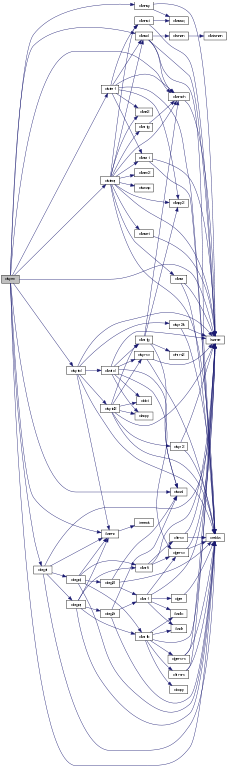
\includegraphics[height=6.5cm]{callg_dsyev.png} 
%\caption{Callgraph xSYEIGV.}
\end{center}
\end{figure}
%
\end{columns}
\end{frame}%}}}
\begin{frame} %{{{
\frametitle{THE SVD ALGO:}
\begin{itemize}
	\item <1-> Definition: 
		%\begin{enumerate} %..
		%	\item
				The singular values of the matrix $A\in\mathbb C^{n\times m}$ is the 
				square root of the eigenvalues of the square symmetric matrices $A^TA$.% and $AA^T$.
		%  	\item
		%		The columns of $U$ are called the left singular vectors of $A$ and the columns and the 
		%		columns of $V$ are called the right singular vectors of $A$.
		%\end{enumerate}
\end{itemize}
		\begin{theorem} <2->
			(The Singular Value Decomposition:)
			Let $A$ be an $m\times n$ complex matrix of rank $r$. Then there exist an $m\times m$
			orthogonal matrix $U$, an $n\times n$ orthogonal matrix $V$ and an $n\times m$ diagonal 
			matrix $\Sigma$ such that 
			\begin{equation}
				A = U \Sigma V^\dagger,
			\end{equation}
			where $\diag (\Sigma) = (\sigma_1,\sigma_2,\dots,\sigma_r, 0,0,\dots,0,)$ and 
			$\sigma_1\ge\sigma_2\dots\ge\sigma_r\ge0$.
		\end{theorem}
\end{frame}%}}}
\begin{frame}%{{{
\frametitle{THE SVD ALGO:}
\begin{itemize}
	\item <1-> The following procedure will produce a SVD-factorization of $A$. 
		\begin{enumerate}
			\item Form $C=A^\dagger A$.
			\item Use the Symmetric QR - Algorithm to find 
				$V^\dagger CV = \diag{(\sigma_{1}^2,\sigma_{2}^2,\cdots,\sigma_{m}^2)}$
			\item Apply QR with column pivoting to $AV$  obtaining $U^T(AV)\Pi=R$.
		\end{enumerate}
	\item <2-> Now  $(U\Pi)^T A V = \Sigma$ is the SVD since:
		\begin{enumerate}
			\item $U$ is orthogonal and $AV$ have orthogonal columns. Then $R$ is diagonal.  
				(It is easy to show that for a triangular matrix to be orthogonal it must be diagonal).
			\item $V$ is orhogonal.
		\end{enumerate}
	\item <3-> Problem: unwise to multiply $A,\,A^\dagger$ since small elements  
		$A_{ij}<\sqrt{\ts u}$ will disappear due to round off error.
\end{itemize}
\end{frame}%}}}
\begin{frame}%{{{
	\frametitle{THE SVD ALGO}
	\begin{itemize}
		\item <1-> Multiplication $A^\dagger A$ be ommitted:
			\begin{enumerate}
				\item Reduce $A$ to real bidiagonal form via a Householders reduction s.t. 
					\begin{align}
						U_B^T A V_B = \smatrix{B\\0} ,\, B = 
						\smatrix{
							d_1 & t_1 & & & 0\\
							0 & d_2 & t_2 & & \\
							& 0 & d_3 & \ddots & \\
							& & \ddots	& \ddots & t_{n-1} \\
							0& & & 0& d_n 
						}
					\end{align}
					This is a $\mathcal O(mn^2)$ operation, assuming that $m\ge n$).
		\item <2-> The matrix $B^TB$ is real and tridiagonal and can be unitarily transformed to a diagonal matrix 
						$\diag (\sigma_1^2, \sigma_2^2,\dots, \sigma_n^2)$ using the symmetric $QR$ algorithm.
			\end{enumerate}
	\end{itemize}
\end{frame}%}}}
\begin{frame}%{{{
\frametitle{THE SVD ALGO}
\begin{itemize}
	\item In the implicit QR-algorithm we would:
		\begin{enumerate}
			\item
				do a implicit QR-step with the Wilkinson shift of the last block of $B^TB$
				\begin{align}
					[B^TB](n-1:n,n-1:n) = \smatrix{d^2_{n-1}+f^2_{n-2} & d_{n-1}f_{n-1} \\ d_{n-1}f_{n-1} & d^2_n+f^2_{n-1}}
				\end{align}
				(The eigenvalue that is closest to $d^2_n+f^2_{n-1}$), 
			\item and compute the first givens rotation $V_1=\smatrix{G_1 & 0 \\ 0 & I}$ with the restraint that $Ve_1=Qe_1$.
			\item Find the $V_2,V_3,\dots$ that brings $V_1B^TBV_1$ back to tridiagonal form 
			\item and set
				\begin{align}
					B^TB \gets V^TB^TBV
				\end{align}
		\end{enumerate}
\end{itemize}
\end{frame}%}}}
\begin{frame}%{{{
	\frametitle{THE SVD ALGO}
	\begin{itemize}
		\item <1->  The multiplication $B^TB$ can also be ommited, using a strategy similar to that of the implicit QR-algorithm.
			\begin{enumerate}
				\item $5\times 5$ example:
					\begin{equation}
						\begin{footnotesize}
							T'= T V_1= 
							\smatrix
							{
								\times 	& \times & 0 & 0 & 0   \\
								+ 	& \times & \times & 0 & 0   \\
								0 & 0 & \times & \times & 0   \\
								0 & 0 & 0 & \times & \times     \\
								0 & 0 & 0 & 0 & \times    \\
							}
							,\,
							T''=  U_1^T T'  = 
							\smatrix
							{
								\times 	& \times & + & 0 & 0   \\
								0	& \times & \times & 0 & 0   \\
								0 	& 0 & \times & \times & 0    \\
								0 & 0 & 0 & \times & \times   \\
								0 & 0 & 0 & 0 & \times  \\
							}
						\end{footnotesize}
					\end{equation}
		%,\notag\\
					\begin{equation}
						\begin{footnotesize}
							U'''= T'' V_2 = 
							\smatrix
							{
								\times 	& \times & 0 & 0 & 0   \\
								0 	& \times & \times & 0 & 0   \\
								0 	& + & \times & \times & 0\\
								0 & 0 & 0 & \times & \times   \\
								0 & 0 & 0 & 0 & \times  \\
							}
							,\,
							T''''= U_2^TT'''= 
							\smatrix
							{
								\times 	& \times & 0 & 0 & 0   \\
								0 	& \times & \times & + & 0   \\
								0 	& 0 & \times & \times & 0    \\
								0 & 0 & 0 & \times & \times   \\
								0 & 0 & 0 & 0 & \times  \\
							}
						\end{footnotesize}
					\end{equation}
					and so on... 
				\item After $2n-2$ iterations the matrix will be back on bidiagonal form.
			\end{enumerate}
		\item <2-> Since $(U^T B V)U^T B V = V^T(B^TB)V = \tilde B^T\tilde B$ is tridiagonal, 
			it follows from the implicit-Q theorem that $V$ is essentially the same matrix that we would use
			the QR-iteration step.
		\item <3-> $B$ will converge to diagonal form with the singular values on the diagonal ($\pm$?).
	\end{itemize}
\end{frame}%}}}
\begin{frame}%{{{
\frametitle{THE SVD ALGO}
\begin{itemize}
	\item The implicit Q-theorem only holds if the tridiagonal matrix is unreduced. 
	\item We must have this in mind when we diagonalize $B$. 
		\begin{enumerate}
			\item
				If one of the off diagonal element $f_k=0$ the problem decouples into two smaller:
				\begin{align}
					B = 
					\begin{matrix}
						\smatrix{B_1 & 0 \\ 0 & B_2}
					\end{matrix}
				\end{align}
			\item If one of the diagonal elements $d_k=0, k<n$ then we can zero an entire row in $B$
				\begin{footnotesize}
				\begin{align}
						&\smatrix
						{
							1 	& 0 & 0 & 0 & 0   \\
							0 	& c & s & 0 & 0   \\
							0 	& -s & c & 0 & 0    \\
							0 & 0 & 0 & 1 & 0   \\
							0 & 0 & 0 & 0 & 1  \\
						}
						\smatrix
						{
							\times 	& \times & 0 & 0 & 0   \\
							0 	& 0 & \times & 0 & 0   \\
							0 	& 0 & \times & \times & 0    \\
							0 & 0 & 0 & \times & \times   \\
							0 & 0 & 0 & 0 & \times  \\
						}
						=
						\smatrix
						{
							\times 	& \times & 0 & 0 & 0   \\
							0 	& 0 & 0 & + & 0   \\
							0 	& 0 & \times & \times & 0    \\
							0 & 0 & 0 & \times & \times   \\
							0 & 0 & 0 & 0 & \times  \\
						}\\
						&\smatrix
						{
							1 & 0 & 0 & 0 & 0   \\
							0 & c & 0 & s & 0   \\
							0 & 0 & 1 & 0 & 0    \\
							0 & -s & 0 & c & 0   \\
							0 & 0 & 0 & 0 & 1  \\
						}
						\smatrix
						{
							\times 	& \times & 0 & 0 & 0   \\
							0 	& 0 & 0 & + & 0   \\
							0 	& 0 & \times & \times & 0    \\
							0 & 0 & 0 & \times & \times   \\
							0 & 0 & 0 & 0 & \times  \\
						}
						=
						\smatrix
						{
							\times 	& \times & 0 & 0 & 0   \\
							0 	& 0 & 0 & 0 & +   \\
							0 	& 0 & \times & \times & 0    \\
							0 & 0 & 0 & \times & \times   \\
							0 & 0 & 0 & 0 & \times  \\
						}\\
						&\smatrix
						{
							1 & 0 & 0 & 0 & 0   \\
							0 & c & 0 & 0 & s   \\
							0 & 0 & 1 & 0 & 0    \\
							0 & 0 & 0 & 1 & 0   \\
							0 & -s & 0 & 0 & c  \\
						}
						\smatrix
						{
							\times 	& \times & 0 & 0 & 0   \\
							0 	& 0 & 0 & 0 & +   \\
							0 	& 0 & \times & \times & 0    \\
							0 & 0 & 0 & \times & \times   \\
							0 & 0 & 0 & 0 & \times  \\
						}
						=
						\smatrix
						{
							\times 	& \times & 0 & 0 & 0   \\
							0 	& 0 & 0 & 0 & 0   \\
							0 	& 0 & \times & \times & 0    \\
							0 & 0 & 0 & \times & \times   \\
							0 & 0 & 0 & 0 & \times  \\
						}
				\end{align}
				This situation corresponds to a degeneracy in the eigenvalues since $B^TB$ in this case have
				a $2\times 2$ block with equal elements in the upper left block of $B^TB$.
				\end{footnotesize}
			\item If $k=n$ we can zero the last column using a similar strategy using column rotations (multiplying with the givens rotations from the right).
				\item Both situations corresponds to a decoupled problem $B^TB=\smatrix{T_1&0 \\ 0&T_2}$.
		\end{enumerate}
\end{itemize}
\begin{Tiny}
	((note that $U^TB^TBU$ and $V^TB^TBV$ both has the same singular values on the diag)).
\end{Tiny}
\end{frame}%}}}
\begin{frame}%{{{
\frametitle{THE SVD ALGO}
\begin{algo}[The SVD Algorithm]
	\begin{footnotesize}
		\textbf{Input: }
		{
%
			The general matrix $A\in\mathbb R^{m\times n}$,
%
		}
		\textbf{Output: }
		{
%
			Overwrites $A$ with $U^TAV=D+E$ where $D$ is diagonal and $\norm E_{2} \approx \ts u \norm{E}_{2}$ and
			$U\in\mathbb R^{m\times n},\, V\in\mathbb R^{m\times m}$ are orthogonal.
%
		}\\
		\line(1,0){120}
		\begin{algorithmic}
%
			\State{Compute the bidiagonalization $\smatrix{B\\0}\gets(U_1\dots U_{n})^TA(V_1\dots V_n-2))$}
			\While{$q\le n$}
			\For{$i=1:n-1$}
				\If{$|b_{i,i+1}|\le\epsilon(|b_{ii}|+|b_{i+1,i+1}|)$}
					\State{$b_{i,i+1}\gets0$}
				\EndIf{}
			\EndFor{}
			\State{Find the largest $q$ and the smallest $p$ such that if
				\begin{equation*}
					D = 
					\begin{matrix}
						\\
						\smatrix{B_{11} & 0 & 0 \\ 0 & B_{22} & 0 \\ 0 & 0 & B_{33}} 
						& 
						\begin{matrix}
							p \\ n-p-q \\ q
						\end{matrix}
						\\
						\begin{matrix}
							p & n-p-q & q
						\end{matrix}
					\end{matrix},
				\end{equation*}
			}
			\State{then $B_{33}$ is diagonal and $B_{22}$ has a nonzero superdiagonal}
			\If{$q<n$}
				\If
					\State{if any subdiagonal iz zero, then zero the superdiagonal endry on the same row}
				\Else{}
					\State{Apply the Golub-Kahan step on $D_{22}:$}
					\State{\hspace{4mm}$B=\text{diag}(I_p, U, I_{q+m-n})^T B\text{diag}(I_p, V, I_q) $}
				\EndIf{}
			\EndIf{}
			\EndWhile{}
%
		\end{algorithmic}
		\label{algSVDAlgorithm}
		\line(1,0){120}
	\end{footnotesize}
\end{algo}
\end{frame}%}}}
\begin{frame}%{{{
\frametitle{LAPACK AND SVD}
\begin{itemize}
	\item In the first step, the matrix is reduced to a bidiagonal matrix 
		(xGEBRD or xGBBRD for banded matrices).
	\item The second step is to compute the SVD of the bidiagonal matrix. 
		%This takes O(mn2) floating-point operations (flops), assuming that m ≥ n (this formulation uses the big O notation). 
		%The second step takes O(n) iterations, each costing O(n) flops. Thus, the first step is more expensive, and the overall cost is O(mn2) flops (Trefethen & Bau III 1997, Lecture 31).
		Lapack uses two different strategies, where the second is much faster with multithreading.
		\begin{enumerate}
			\item Small matrices: A variant of the Golub-Kahan Algorithm (xBDSQR).
			\item Large matrices: A variant of Divide-and-conquer $+$ Golub-Kahan (xBDSDC)
		\end{enumerate}
	\item $+$ a huge amounts of technicalities and optimizations.
\end{itemize}
\end{frame}%}}}
\begin{frame}%{{{
\frametitle{LAST SLIDE:}
	\begin{bf}
		\begin{large}
			\begin{center}
				Thank you for the attention!
				\nocite{*}
			\end{center}
		\end{large}
	\end{bf}
\end{frame}%}}}
\begin{frame}[label=householders explained] \frametitle{Householders reflections explained}%{{{
		\begin{itemize}
			\item A Householder reflection is a rank 1 matrix on the form $H_1 = I - 2\frac{uu^T}{u^Tu}$.
			\item To find a Householder matrix such that $H_1 x \propto e_1$ we choose $u = x \pm \norm{x}_2 e_1$.
				Then $H_1 x = \pm \norm{x}_2 e_1$.
			\item If the $n\times n$ matrix $A$ can be written on the form \[ A = \smatrix{a_{11} & x^T \\ x & A(2:n,2:n)} \] 
				and \[H = \smatrix{1 & 0 \\ 0 & H_1} \] then
				\[ HAH = \smatrix{a_{11} & \pm \norm{x}_2 e_1^T \\ \pm \norm{x}_2 e_1 &  H_1A(2:n,2:n)H_1 }\]
			\item The rest of the matrix can be systematically reduced to tridiagonal form by constructiong the $n-2\times n-2$ matrix $H_2$
				to remove the sub sub diagonal elements of the second column in the same manner, and so on.
			\item Hermitian matrices can be reduced to tridiagonal real and symmetric form (or real bidiagonal form ($H_aAH_b$)). General matrices can be brought to Hessenberg form.
		\end{itemize}
		\hyperlink{tridiagonalizationofa}{\beamergotobutton{return}}
	\end{frame}%}}}
\begin{frame}[label=dist span] \frametitle{Distance between two subspaces}%{{{
\begin{itemize}
	\item Assume $A = [a_1, a_2, \dots, a_m],\, B = [b_1, b_2, \dots, b_m]$ are orthogonal matrices.
	\item Then
		\[ \text{dist}(\text{span}(a_1,\dots,a_m), \text{span}(b_1,\dots,b_m)
			= \norm{A-B}_2
			\]
			which is the modulus of the eigenvalue of the matrix $A-B$ with the largest modulus.
		\item
			When the overlap between the subspaces increase, 
			$\text{dist}(\text{span}(b_1,\dots,b_m), \text{span}(b_1,\dots,b_m)$
			will decrease.
	\end{itemize}
	\begin{tiny}
		Example:
		$A = a_1a_1^T + a_2a_2^T\in\mathbb R^2$, $B = b_1b_1^T + b_2b_2^T \in\mathbb R^2$. $A_H = a_1a_1^T + a_2a_2^T + a_3a_3^T 
		\in\mathbb R^3$, $A_H^TA_H=I$.
		\begin{align}
			\norm{A-B}_2 
			&= \norm{A-A_H^TA_HBA_H^TA_H}_2 \\
			&= \lVert a_1a_1^T ( 1 - a_1^Tb_1b_1^Ta_1 - a_1^Tb_1b_1^Ta_1 )\notag\\
			&+ 	a_2a_2^T ( 1 - a_2^Tb_1b_1^Ta_2 - a_2^Tb_2b_2^Ta_2 )\notag\\
			&+ 	a_3a_3^T(- a_3^Tb_1b_1^Ta_3 - a_3^Tb_1b_1^Ta_3) \rVert_2
		\end{align}
		Note that $a_i^Tb_jb_j^Ta_i\in[0,1]$.
		The distance is is $\text{max}
		( |1 - a_1^Tb_1b_1^Ta_1 - a_1^Tb_1b_1^Ta_1 |,
		|1 - a_2^Tb_1b_1^Ta_2 - a_2^Tb_2b_2^Ta_2 |,
		|- a_3^Tb_1b_1^Ta_3 - a_3^Tb_1b_1^Ta_3|).$
		Which is $0$ only in the case that $A=B$.\\
	\end{tiny}
	\hyperlink{framelb1}{\beamergotobutton{return}}
\end{frame}%}}}
\bibliographystyle{plain}	% (uses file "plain.bst")
\bibliography{qr_art}		% expects file "qr_art.bib"

\end{document}
% vim:foldmethod=marker
